\section{Lecture 4: Wave Packets}

\subsection{Aside: The Fourier Transform}
First let us define the Discrete Fourier Transform.

\begin{theorem}[Discrete Fourier Transform]
    Suppose you have a periodic function $f$ such that $f(x + 2\pi) = f(x)$ for all $x$. If we want to write
    \[ f(x) = \frac{1}{2} A_0 + \sum_{n = 1}^{\infty} (A_n \cos(nx) + B_n \sin(nx)) \]
    We can do so by setting:
    \begin{align*}
        A_n &= \frac{1}{\pi} \int f(x) \cos(nx) \dd{x} \\
        B_n &= \frac{1}{\pi} \int f(x) \sin(nx) \dd{x}
    \end{align*}
\end{theorem}

How can we show this?
Just like with a cartesian vector space, we can use inner products to project onto a basis of functions.
What is the inner product for functions? It is the integral of the ordinary product:
\begin{align*}
    \langle f(x), g(x) \rangle &= \frac{1}{\pi} \int f(x) g(x) \dd{x}
\end{align*}
Thus:
\begin{align*}
    A_m &= \langle f(x), \cos(mx) \rangle \\
    B_m &= \langle f(x), \sin(mx) \rangle
\end{align*}

Now, suppose you want to decompose your function as:
\[
    f(x) = \frac{1}{\sqrt{2\pi}} \sum_{n = -\infty}^{\infty} c_n e^{inx}
\]
Then (by a similar projection argument):
\[ c_m = \frac{1}{\sqrt{2\pi}} \int_{-\pi}^{\pi} f(x) e^{-imx} \dd{x} \]

\begin{definition}[Kronecker Delta]
    The kronecker delta $\delta_{m n}$ is the indicator:
    \[ \delta_{mn} = \begin{cases}
        1 & \text{if $m = n$} \\
        0 & \text{otherwise}
    \end{cases} \]
\end{definition}

Thus we must have,
\begin{theorem}
    The basis functions $e^{inx}$ are orthonormal, i.e.
    \[ \frac{1}{2\pi} \int_{-\pi}^{\pi} e^{i(n - m) x} \dd{x} = \delta_{mn} \]
\end{theorem}

\begin{theorem}[Continuous Fourier Transform]
    If you wish to write:
    \[ f(x) = \frac{1}{\sqrt{2 \pi}} \int_{-\infty}^{\infty} g(k) e^{i kx} \dd{x} \]
    (where $g(k)$ is the continuous fourier transform of $f(x)$), then we have:
    \[ g(k) = \frac{1}{\sqrt{2 \pi}} \int_{-\infty}^{\infty} f(x) e^{-ikx} \dd{x} \]
\end{theorem}

We call these fourier transforms unitary transforms since they change basis but do not lose information.
Let us now explore the continuous version of the delta, the Dirac delta. Plugging in the Fourier transform into the synthesis equation:
\begin{align*}
    f(x) &= \frac{1}{2 \pi} \int_{-\infty}^{\infty} \qty(\int_{-\infty}^{\infty} f(x') e^{-ikx'} \dd{x'}) e^{ikx} \dd{k} \\
    &= \int_{-\infty}^{\infty} f(x') \delta(x - x') \dd{x}
\end{align*}
where we define:
\begin{definition}[Dirac Delta]
    The dirac delta distribution is defined as:
    \[ \delta(y) = \frac{1}{2\pi} \int_{-\infty}^{\infty} e^{iky} \dd{k} \]
\end{definition}
Some wacky properties:
\begin{itemize}
    \item $\delta(x - x') = 0$ if $x \neq x'$
    \item $\int_{\text{region including }0} \delta(x) \dd{x} = 1$ otherwise
\end{itemize}
Notice something interesting, a single frequency, a single $\delta$ is infinitely thin! But if you take up more frequencies in the frequency domain, add together more and more $\delta$s,
the time and space components of the wave will be thinner!

\subsection{Wave Packets and Normalization}
By probability density laws,
\[ \int{\mathbb{R}^3} |\Psi(\mbf{r}, t)|^2 \dd{\mbf{r}} = 1 \]
but for this basic wave that spans all of space, this diverges! (Or the wavefunction is zero everywhere). Instead we have
wave packets that are much more localized.

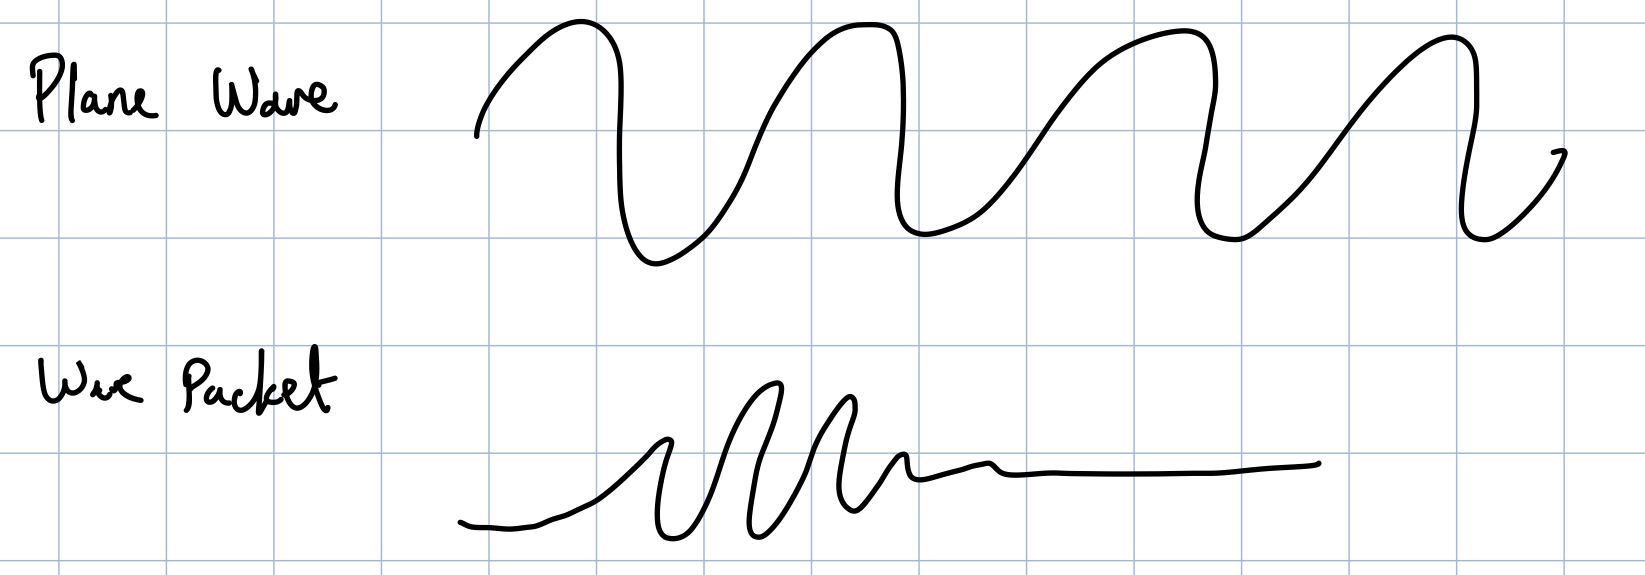
\includegraphics[width=400px]{../images/wave_packet.jpeg}

Suppose we have some waves indexed by $j$: $A_j e^{i (k_j x - \omega t)}$. We want to pick them and add them up to get this localized shape.

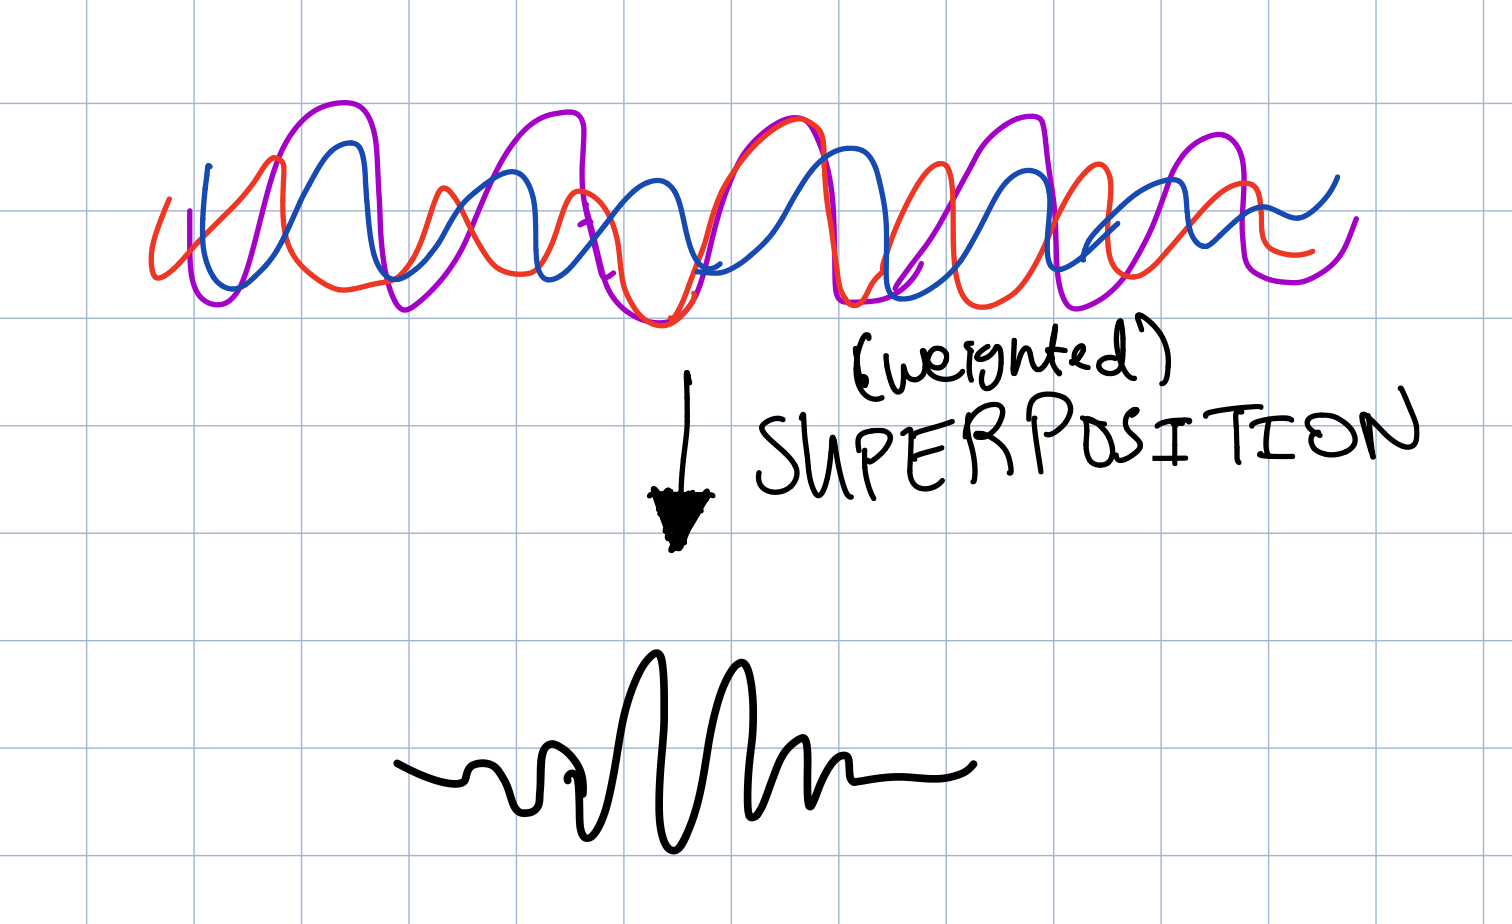
\includegraphics[width=400px]{../images/fourier_sup.jpeg}

For a 1-D wavepacket, the wave function is as follows (our index $j$ has become continuous $p_x$).
\[ \Psi(x, t) = \frac{1}{\sqrt{2 \pi \hbar}} \int e^{\frac{i(p_x x - Et)}{\hbar}} \phi(p_x) \dd{p_x} \]
Let us assume $\phi(p_x)$ is a sharp (non-delta) function that is centered $p_0$ and has half-max width $2 \delta p_x$.

Let
\[ \beta(p_x) = p_x x - E(p_x) t \]
Then
\[ \Psi(x, t) = \frac{1}{\sqrt{2 \pi \hbar}} \int e^{\frac{i\beta(p_x)}{\hbar}} \phi(p_x) \dd{p_x} \]
In the vicinity of $p_0$ is the only place where the integral does not vanish. Furthermore, we also do not want the exponential to rapidly oscillate (this will kill the integral)
so we only get nonzero components in places where $\beta(p_x)$ doesn't vary much. Thus we look for the stationary phase condition
\[ \derivative{\beta(p_x)}{p_x} \Bigl|_{p_x = p_0} = 0 \]
So, doing this yields:
\begin{align*}
    x - t \derivative{}{p_x} E(p_x) &= 0 \\
    \frac{x}{t} &= \derivative{E(p_x)}{p_x}
\end{align*}
where this quantity is defined as the group velocity $v_g$. This is how fast the highest amplitude part of the wave packet moves:

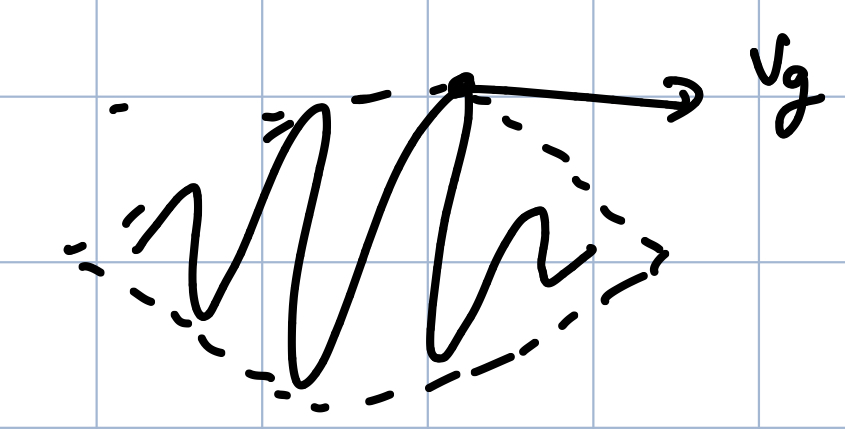
\includegraphics[width=200px]{group_vel.jpeg}

We can also find the phase velocity, the velocity of each component. Each component is:
\begin{align*}
    &e^{i(k_0 x - \omega(k_0) t)} \\
    k_0 x - \omega(k_0)t &= 0 \\
    v_p &= \frac{x}{t} = \frac{E(p_0)}{p_0}
\end{align*}

